\documentclass[11pt,a4paper]{article}
\usepackage[T1]{fontenc}
\usepackage[utf8]{inputenc}
\usepackage{lmodern}
\usepackage[margin=2.5cm]{geometry}
\usepackage{booktabs}
\usepackage{tabularx}
\usepackage{array}
\usepackage{longtable}
\usepackage{xcolor}
\usepackage{enumitem}
\usepackage{fancyhdr}
\usepackage{titlesec}
\usepackage{listings}
\usepackage{float}
\usepackage{amssymb}
\usepackage{tikz}
\usetikzlibrary{positioning,arrows.meta,calc,decorations.pathreplacing}
\usepackage{xurl}
\usepackage{hyperref}

\hypersetup{colorlinks=true, linkcolor=blue!50!black, urlcolor=blue!50!black}

\definecolor{codebg}{gray}{0.96}
\definecolor{notebg}{RGB}{255,246,228}
\definecolor{noteframe}{RGB}{200,110,0}
\definecolor{tipbg}{RGB}{232,242,252}
\definecolor{tipframe}{RGB}{42,120,214}
\definecolor{okgreen}{RGB}{0,120,60}
\definecolor{kw}{RGB}{0,70,150}
\definecolor{cm}{RGB}{90,110,90}

\lstdefinelanguage{VHDLx}{
  morekeywords={library,use,entity,is,port,in,out,inout,end,architecture,of,begin,signal,constant,variable,
    process,if,then,elsif,else,wait,until,for,loop,while,report,severity,assert,generic,map,type,function,
    return,package,body,when,others,downto,to,not,and,or,file,generate,exit,procedure},
  sensitive=false, morecomment=[l]{--}, morestring=[b]"}
\lstset{
  basicstyle=\ttfamily\small,
  backgroundcolor=\color{codebg},
  frame=single,
  rulecolor=\color{gray!40},
  breaklines=true,
  columns=fullflexible,
  keepspaces=true,
  showstringspaces=false,
  keywordstyle=\color{kw}\bfseries,
  commentstyle=\color{cm}\itshape,
  upquote=true
}

\newcommand{\code}[1]{\texttt{#1}}
\newcommand{\bs}{\textbackslash\allowbreak{}}
\let\oldunderscore\_
\renewcommand{\_}{\oldunderscore\allowbreak{}}
\newcommand{\pld}[1]{\code{C:\bs PLD\bs #1}}
\newcommand{\menu}[1]{\textsf{#1}}
\newcommand{\checkbox}{$\square$\ }
\newcolumntype{Y}{>{\raggedright\arraybackslash}X}

\newcommand{\important}[1]{%
  \par\smallskip\noindent
  \fcolorbox{noteframe}{notebg}{\parbox{\dimexpr\linewidth-2\fboxsep-2\fboxrule\relax}{\small\textbf{Important.} #1}}%
  \par\smallskip}
\newcommand{\tip}[1]{%
  \par\smallskip\noindent
  \fcolorbox{tipframe}{tipbg}{\parbox{\dimexpr\linewidth-2\fboxsep-2\fboxrule\relax}{\small\textbf{Tip.} #1}}%
  \par\smallskip}
\newcommand{\why}[1]{%
  \par\smallskip\noindent
  \fcolorbox{tipframe}{tipbg}{\parbox{\dimexpr\linewidth-2\fboxsep-2\fboxrule\relax}{\small\textbf{Why.} #1}}%
  \par\smallskip}
\newcommand{\say}[1]{%
  \par\smallskip\noindent
  \fcolorbox{okgreen}{green!5}{\parbox{\dimexpr\linewidth-2\fboxsep-2\fboxrule\relax}{\small\textbf{What to say.} #1}}%
  \par\smallskip}

\setlength{\emergencystretch}{3em}
\setlength{\parskip}{4pt}
\setlength{\parindent}{0pt}
\titleformat{\subsection}{\normalfont\large\bfseries}{\thesubsection}{1em}{}
\pagestyle{fancy}
\fancyhf{}
\lhead{\small TeraNova -- FPGA Acceleration}
\rhead{\small Rung simulation guide -- K.~Janssen (4994817)}
\cfoot{\small\thepage}
\renewcommand{\headrulewidth}{0.4pt}

\begin{document}

\begin{titlepage}
\centering
\vspace*{3cm}
{\LARGE\bfseries Rung Simulation Guide\par}
\vspace{0.5cm}
{\Large Showing the Improvement Ladder\\in the Vivado Simulator\par}
\vspace{0.3cm}
{\large TeraNova -- FPGA Acceleration\par}
\vspace{2cm}
\begin{tabular}{@{}ll@{}}
\textbf{Author}   & Kai Janssen (4994817) \\
\textbf{Version}  & 5 November 2026 \\
\textbf{Tools}    & Vivado 2025.1.1 (Vivado simulator, XSim), no licence needed \\
\textbf{Files}    & \code{C:\bs PLD\bs sim\bs vivado} \\
\textbf{Companion}& \emph{Vivado Simulation Guide} (how XSim works) \\
\end{tabular}
\vfill
{\small All cycle counts in this guide were checked by running the same VHDL with GHDL before the guide was written; they are identical to \code{sim\bs ladder.md}.\par}
\end{titlepage}

\tableofcontents
\newpage

% ==================================================================
\section{What you will show}
% ==================================================================
One Vivado simulation that runs \textbf{all five rungs side by side}: five copies of the PL data path, each with the RTL of one rung, on the same 100\,MHz clock, started by the same start pulse at the same moment. Every rung multiplies the same two $50\times50$ matrices and checks its own result. In the wave window you then see directly:

\begin{itemize}[nosep]
  \item how much sooner each rung finishes (one \code{busy} bar per rung, markers at every \code{done});
  \item \emph{why} it is faster, by zooming into the blocks: the partitioner state machine, the BRAM addresses, the handshakes between the blocks and the AXI write and read channels;
  \item that every rung still computes the right answer (the summary table in the Tcl Console).
\end{itemize}

\begin{table}[H]
\centering\small
\begin{tabularx}{\textwidth}{@{}clrrrY@{}}
\toprule
\textbf{Rung} & \textbf{Change} & \textbf{L = 20} & \textbf{vs prev.} & \textbf{L = 100} & \textbf{What you see in the waves} \\
\midrule
0 & baseline (restored design) & 101\,186 & -- & 101\,586 & 4 cycles per element, 101 cycles per block pair \\
1 & partitioner v5b & 27\,186 & 3.72$\times$ & 58\,576 & a new BRAM address every cycle, 27 cycles per pair \\
2 & writer fix & 27\,071 & 1.00$\times$ & 27\,151 & writes no longer wait for each response (gain shows at L = 100: 2.15$\times$) \\
3 & partitioner v6 & 10\,052 & 2.69$\times$ & 18\,052 & one load phase, then a block pair every 6 cycles \\
4 & burst data path & 10\,073 & 1.00$\times$ & 18\,153 & PL reads A and B itself in 4\,KB AXI bursts \\
\bottomrule
\end{tabularx}
\caption{Expected PL run time (clock cycles from start to \code{done}, 10\,ns each) for memory latency $L = 20$ (nominal) and $L = 100$ (stress). Rung 0 to rung 3 at $L = 20$: 10.06$\times$ faster.}
\label{tab:expected}
\end{table}

\important{Rung 4 is \emph{not} faster in this simulation, and that is correct: its gain is on the \textbf{CPU} side (no more 10\,000 single CPU writes into the BRAMs and 2\,500 uncached reads, estimated at 2.25\,ms of the 2.35\,ms end-to-end). A PL simulation cannot show CPU time. Say this before your tutor asks; it shows you understand where the time goes.}

% ==================================================================
\section{How the simulation is built}
% ==================================================================

\begin{figure}[H]
\centering
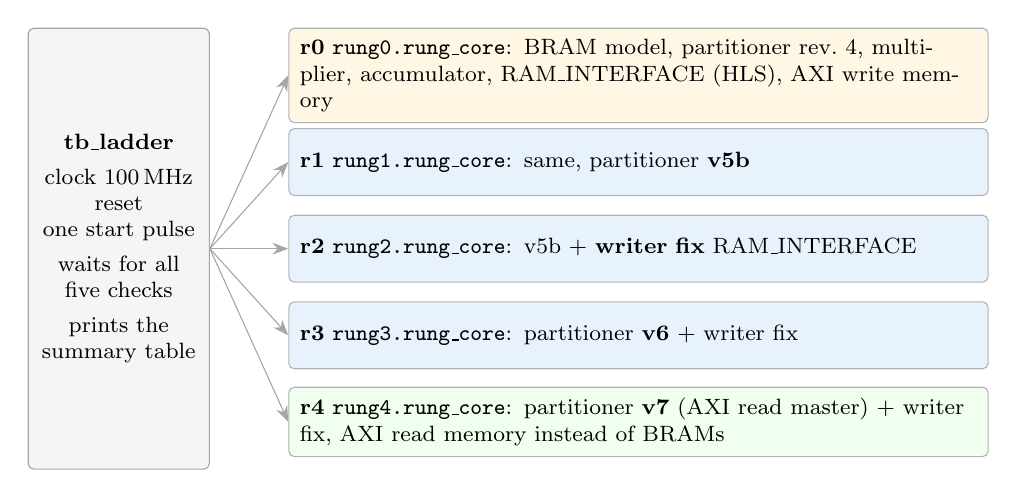
\begin{tikzpicture}[
  rung/.style={draw=gray!60, rounded corners=2pt, fill=#1, align=left, text width=8.6cm, minimum height=0.85cm, inner sep=4pt, font=\footnotesize},
  arr/.style={-{Stealth[length=2mm]}, gray!70}]
\node[draw=gray!70, fill=gray!8, rounded corners=2pt, align=center, minimum width=2.3cm, minimum height=5.6cm, font=\footnotesize] (tb) at (0,0) {\textbf{tb\_ladder}\\[3pt]clock 100\,MHz\\reset\\one start pulse\\[3pt]waits for all\\five checks\\[3pt]prints the\\summary table};
\node[rung=notebg] (r0) at (6.6, 2.2) {\textbf{r0} \code{rung0.rung\_core}: BRAM model, partitioner rev.~4, multiplier, accumulator, RAM\_INTERFACE (HLS), AXI write memory};
\node[rung=tipbg]  (r1) at (6.6, 1.1) {\textbf{r1} \code{rung1.rung\_core}: same, partitioner \textbf{v5b}};
\node[rung=tipbg]  (r2) at (6.6, 0.0) {\textbf{r2} \code{rung2.rung\_core}: v5b + \textbf{writer fix} RAM\_INTERFACE};
\node[rung=tipbg]  (r3) at (6.6,-1.1) {\textbf{r3} \code{rung3.rung\_core}: partitioner \textbf{v6} + writer fix};
\node[rung=green!6](r4) at (6.6,-2.2) {\textbf{r4} \code{rung4.rung\_core}: partitioner \textbf{v7} (AXI read master) + writer fix, AXI read memory instead of BRAMs};
\foreach \r in {r0,r1,r2,r3,r4} \draw[arr] (tb.east) -- (\r.west);
\end{tikzpicture}
\caption{Structure of the simulation. Each rung is compiled into its own VHDL library, so the five partitioners and the two \code{RAM\_INTERFACE} versions can keep the same entity names.}
\label{fig:structure}
\end{figure}

\subsection{What is the real design and what is testbench}
\begin{itemize}[nosep]
  \item \textbf{Design RTL, unchanged}: the multiplier (\code{MatMul5x5}, \code{MatMul5x5\_IF\_IN}), the accumulator, \code{matrix\_to\_ports}, the partitioners (\code{matrix\_partitioner\_B.vhd} and \code{variants\bs *\_v5b/v6/v7.vhd}) and the \textbf{real Vitis-HLS RTL} of \code{RAM\_INTERFACE} (\code{hls\_rtl} and \code{steps\bs 2\_writer\_fix\bs hls\_rtl}). The scripts take them straight from \pld{sim}, the same files that \code{ladder.json} uses.
  \item \textbf{Testbench}: \code{rung\_core} is a copy of \code{tb\_chain\_rtl.vhd} (rung 4: \code{tb\_chain\_axi.vhd}) with three changes: clock/reset/start come in through ports, the matrices come from a VHDL package instead of \code{a\_b.hex}, and the result is read back from the memory model and compared with the exact product inside VHDL (instead of \code{c\_out.hex} + Python). The memory models are the ones of \pld{sim} with a read-back port added.
  \item \textbf{Data}: the ``hello'' data set of \code{helloworld.c}: $A_{ij} = 50i + j + 1$, $B_{ij} = 50i + j + 2$.
  \item \textbf{Checks per rung}: all 2\,500 words of $C = A\times B$ correct, exactly 100 output blocks (no lost or duplicated blocks), no unexpected AXI reads.
\end{itemize}

\why{The cycle count is measured exactly as in \code{tb\_chain\_rtl}: from the clock edge where the partitioner sees \code{start} until \code{done} of \code{RAM\_INTERFACE}. The new testbench was run with GHDL before it was handed over and gives the same numbers as the ladder runner, for both latencies (Table~\ref{tab:expected}). A check with a deliberately wrong expected value was also run, to confirm that the checker really reports errors.}

% ==================================================================
\section{Tonight: dry run}\label{sec:tonight}
% ==================================================================
Do the whole demo once at home, so tomorrow only things you have already seen can happen.

\begin{enumerate}
  \item[\checkbox] Laptop with \textbf{Vivado 2025.1.1}. No licence and no board needed.
  \item[\checkbox] The folder \pld{sim\bs vivado} exists with \code{create\_ladder\_project.tcl}, \code{ladder\_waves.tcl}, \code{run\_ladder\_batch.bat} and \code{src\bs}. The design files of all rungs must be in \pld{sim}: keep the branch \code{burst-datapath} checked out (the last rung; it contains the files of every earlier rung). It is checked out now.
  \item[\checkbox] Run Section~\ref{sec:steps} once completely and write down how long compile and simulation take on your laptop.
  \item[\checkbox] Walk through the demo of Section~\ref{sec:demo} once; place the zoom ranges yourself.
  \item[\checkbox] Save a backup of the finished run (Section~\ref{sec:backup}).
  \item[\checkbox] Optional: run \code{run\_ladder\_batch.bat} once as a second, independent check.
\end{enumerate}

\tip{The new files in \pld{sim\bs vivado} are not in git yet. If you want them on GitHub (and on Badr's laptop): \code{git add sim/vivado .gitignore} and commit them on \code{burst-datapath} (the branch you are on). The generated folders (\code{project}, \code{lib}, \code{batch}) are already in \code{.gitignore}.}

% ==================================================================
\section{Step by step}\label{sec:steps}
% ==================================================================

\subsection{Create the project}
\begin{enumerate}
  \item Start Vivado 2025.1.1. Do not open a project.
  \item In the \textbf{Tcl Console} at the bottom of the start page type:
\begin{lstlisting}
source C:/PLD/sim/vivado/create_ladder_project.tcl
\end{lstlisting}
  \item The console prints one line per rung and ends with \code{Project created: ...\bs project\bs teranova\_ladder.xpr}. The project is open.
\end{enumerate}

Check in the \textbf{Sources} window, \menu{Simulation Sources > sim\_1}:
\begin{itemize}[nosep]
  \item \code{tb\_ladder} is in \textbf{bold} (the top) and has the instances \code{r0} to \code{r4} below it;
  \item in the \menu{Libraries} tab there are \code{tn\_common}, \code{rung0} \ldots{} \code{rung4} and \code{xil\_defaultlib};
  \item \menu{Design Sources} is empty: this project only simulates. Vivado may show warnings about the empty design or about entities with the same name in different libraries; they do not matter.
\end{itemize}

The script made these settings for you (you can see them in \menu{Simulation Settings}):
\begin{tabularx}{\textwidth}{@{}lY@{}}
\toprule
Top & \code{tb\_ladder} \\
Generic & \code{LAT=20} (memory latency in cycles) \\
File type & all files \code{VHDL 2008}, each rung in its own library \\
Compile order & manual, in the order the files were added (\menu{Automatic Update, Manual Compile Order}) \\
\code{xsim.simulate.runtime} & \code{-all}: run until the testbench ends (about 1.09\,ms simulated) \\
\code{xsim.simulate.log\_all\_signals} & \code{true}: every signal is recorded from time 0 \\
\code{xsim.simulate.tcl.post} & \code{ladder\_waves.tcl}: builds the wave view after the run \\
\bottomrule
\end{tabularx}

\subsection{Run}
\begin{enumerate}
  \item Flow Navigator \menu{SIMULATION > Run Simulation > Run Behavioral Simulation}.
  \item Vivado compiles about 75 files (five rungs), elaborates and runs to the end. This takes a few minutes; the status bar at the top right shows the step.
  \item When it is done, the \textbf{Tcl Console} shows the summary:
\end{enumerate}

\begin{lstlisting}[basicstyle=\ttfamily\fontsize{6.2}{7.4}\selectfont]
==================== TeraNova improvement ladder (Vivado XSim) ====================
AXI memory latency L = 20 cycles, clock 100 MHz (10 ns per cycle)
rung                                 PL cycles   PL time (us)   vs previous   vs baseline   multiplier busy   result
rung 0  baseline                        101186        1011.86         1.00x         1.00x            4.94 %   PASS (2500/2500)
rung 1  partitioner v5b                  27186         271.86         3.72x         3.72x           18.39 %   PASS (2500/2500)
rung 2  writer fix                       27071         270.71         1.00x         3.73x           18.46 %   PASS (2500/2500)
rung 3  partitioner v6 (reuse)           10052         100.52         2.69x        10.06x           64.28 %   PASS (2500/2500)
rung 4  burst data path                  10073         100.73         0.99x        10.04x           64.15 %   PASS (2500/2500)
ALL RUNGS PASS: every rung computed all 2500 result words of C = A x B correctly
===================================================================================
\end{lstlisting}

\begin{enumerate}[resume]
  \item A wave window tab \textbf{TeraNova ladder} opens with the groups of Section~\ref{sec:groups} and five markers \code{rung 0 done} \ldots{} \code{rung 4 done}. Press \menu{Zoom Fit}.
\end{enumerate}

\important{If the wave view did not appear (the console says \code{ladder\_waves: ...}), type \code{source C:/PLD/sim/vivado/ladder\_waves.tcl} in the Tcl Console. Because all signals were logged, the waves still show the whole run. If the simulation stopped at 1000\,ns, the run-time setting was not applied: press \menu{Run All}.}

\subsection{The wave view}\label{sec:groups}
\begin{tabularx}{\textwidth}{@{}lY@{}}
\toprule
\textbf{Group} & \textbf{Contents} \\
\midrule
Overview & \code{rst}, \code{start}; \code{busy rung 0..4} (high from start until \code{done}: \emph{this bar is the PL run time}); \code{cycles rung 0..4} (live cycle counters); \code{all results checked} \\
Rung $n$ $>$ Partitioner & \code{state} (shown by name), BRAM address A (rungs 0--3) or the AXI read channel (rung 4), the block counters \code{i\_blk}, \code{j\_blk}, \code{p\_blk} \\
Rung $n$ $>$ Handshakes & pair valid/ready (partitioner $\rightarrow$ multiplier), product valid (multiplier $\rightarrow$ accumulator), block valid/read (accumulator $\rightarrow$ writer), output blocks written \\
Rung $n$ $>$ Writer & the AXI write channel of \code{RAM\_INTERFACE}: AW, W, B handshakes, \code{awaddr}, \code{awlen}, and \code{done} \\
\bottomrule
\end{tabularx}

Collapse the five rung groups at first (triangle in front of the name), so only the overview is visible. Open one rung group at a time during the demo.

% ==================================================================
\section{The demo, step by step}\label{sec:demo}
% ==================================================================
Times below are simulation times. To zoom to a range, drag in the time ruler above the waves, or zoom in with Ctrl + mouse wheel around the point. Start, reset release and the start pulse are at the very beginning: the start pulse is at about 0.17\,\textmu s.

\subsection{The overview: five rungs, one start}
\textbf{Zoom Fit.} The five \code{busy} bars start together and end at the markers:

\begin{figure}[H]
\centering
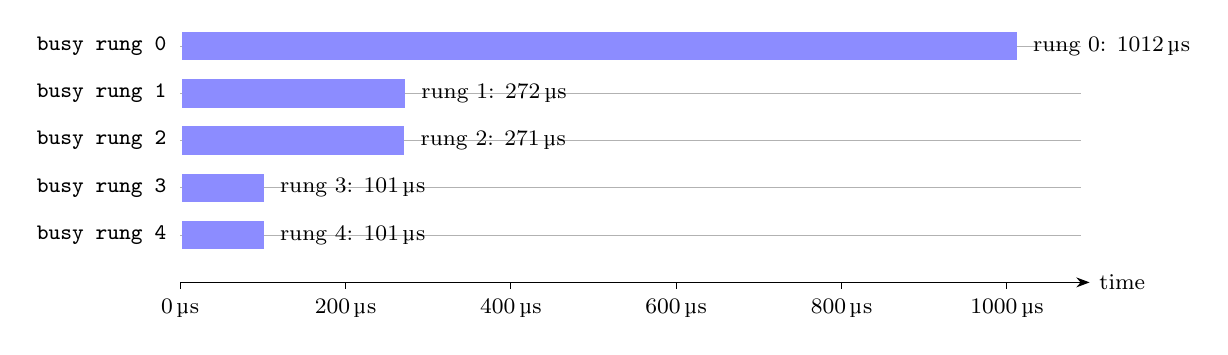
\begin{tikzpicture}[x=0.105mm, y=6mm, font=\footnotesize]
\foreach \n/\c/\l [count=\i from 0] in {0/1012/{rung 0: 1012\,\textmu s}, 1/272/{rung 1: 272\,\textmu s}, 2/271/{rung 2: 271\,\textmu s}, 3/101/{rung 3: 101\,\textmu s}, 4/101/{rung 4: 101\,\textmu s}} {
  \draw[gray!60] (0,-\i) -- (1090,-\i);
  \fill[blue!45] (2,-\i-0.3) rectangle (\c,-\i+0.3);
  \node[anchor=east] at (-5,-\i) {\code{busy rung \n}};
  \node[anchor=west] at (\c+8,-\i) {\l};
}
\draw[-{Stealth}] (0,-5) -- (1100,-5) node[right] {time};
\foreach \t in {0,200,400,600,800,1000} \draw (\t,-5) -- (\t,-5.15) node[below] {\t\,\textmu s};
\end{tikzpicture}
\caption{Sketch of the overview (to scale). The real view is the Vivado wave window.}
\end{figure}

\begin{itemize}[nosep]
  \item Click on a marker label, or on the falling edge of a \code{busy} bar: the \code{cycles rung n} value in the Value column is the PL run time in clock cycles (101\,186, 27\,186, \ldots).
  \item To measure it in time: put a marker on the rising edge of \code{start}, then click on the end of a \code{busy} bar. The distance between cursor and marker is the run time.
\end{itemize}

\say{``These are five versions of our PL data path running in parallel in one simulation, all with the same input and the same start. Each bar is how long that version needs for one 50 by 50 matrix multiplication. The baseline needs 1.01 milliseconds, the last versions 0.10 milliseconds: ten times faster in the PL, and all five produce exactly the right result.''}

\subsection{Rung 0: why the baseline is slow}
Open \textbf{Rung 0 $>$ Partitioner} and \textbf{Handshakes}. Zoom to about 1.0--2.3\,\textmu s.
\begin{itemize}[nosep]
  \item \code{state} goes \code{ISSUE\_ADDR $\rightarrow$ WAIT1 $\rightarrow$ WAIT2 $\rightarrow$ CAPTURE} for every element: the \textbf{BRAM address changes only every 40\,ns = 4 cycles}.
  \item A block pair needs 25 elements: \code{pair valid} pulses every \textbf{1.01\,\textmu s = 101 cycles}.
  \item \code{pair ready} is almost always high: the multiplier, which needs 5 cycles per pair, waits about 95\,\% of the time (``multiplier busy 4.94\,\%'' in the table).
\end{itemize}
\say{``The BRAMs have a read latency of one cycle, but the partitioner spends four cycles per element. The two wait states do nothing. So the expensive single-cycle multiplier is idle 95 percent of the time.''}

\subsection{Rung 1: pipelined fetch}
Open \textbf{Rung 1 $>$ Partitioner} and \textbf{Handshakes}, same zoom range.
\begin{itemize}[nosep]
  \item \code{state} is \code{FETCH} while the 25 elements are read, then briefly \code{OUTPUT}: a new BRAM address \textbf{every cycle (10\,ns)}; each element is captured two edges after its address.
  \item \code{pair valid} every \textbf{270\,ns = 27 cycles} instead of 101. Result: 27\,186 cycles, 3.72$\times$.
\end{itemize}
Tip: put rung 0's and rung 1's \code{BRAM address A} next to each other (drag them into one group) and zoom to about 50\,ns per division: the staircase of rung 0 has steps 4 times as long.

\subsection{Rung 2: the writer fix}
At $L = 20$ rung 2 is only 115 cycles faster, so first show \emph{what} changed. Open \textbf{Writer} of rung 1 and of rung 2 and zoom to about 3.0--3.6\,\textmu s.
\begin{itemize}[nosep]
  \item Every output block ($5\times5$ values) is written as 5 bursts of 5 beats (\code{awlen} = 4), one per row of the block.
  \item \textbf{Rung 1}: the next \code{awvalid} comes only after the \code{bvalid} of the previous burst: one burst every 330\,ns. The writer waits for every write response.
  \item \textbf{Rung 2}: the 5 \code{awvalid}s follow each other every 60\,ns, while the \code{bvalid}s arrive later: the responses overlap with new writes.
\end{itemize}
Then show where it matters, with a higher memory latency (Section~\ref{sec:lat100}): at $L = 100$ rung 1 needs 58\,576 cycles because the writer becomes the bottleneck, rung 2 still 27\,151 (2.15$\times$).
\say{``With a realistic DDR latency the old writer would have eaten most of the gain of rung 1. The fix makes the next rungs independent of a latency we have not measured on the board yet.''}

\subsection{Rung 3: copy once, reuse ten times}
Open \textbf{Rung 3 $>$ Partitioner} and \textbf{Handshakes}; zoom to 0--30\,\textmu s, then into 25--27\,\textmu s.
\begin{itemize}[nosep]
  \item From the start until about 25.2\,\textmu s \code{state} is \code{LOAD}: A and B are copied \emph{once} from the BRAMs into 25 on-chip banks per matrix, one element of each per cycle (about 2\,500 cycles).
  \item After that \code{state} moves through \code{RD}, \code{CAP} and \code{OUTPUT} for every block pair, and \code{pair valid} comes every \textbf{6 cycles}: a whole $5\times5$ block is read from the 25 banks in one cycle.
  \item The multiplier is now busy 64\,\% of the time. Total 10\,052 cycles: 2.69$\times$ faster than rung 2, 10.06$\times$ faster than the baseline.
\end{itemize}

\subsection{Rung 4: the burst data path}
Open \textbf{Rung 4 $>$ Partitioner}; zoom to 0--26\,\textmu s.
\begin{itemize}[nosep]
  \item There are no BRAMs any more: the partitioner itself reads A and B through an \textbf{AXI4 read master}. \code{AXI read ARLEN} = 255 means bursts of 256 beats of 128 bits = 4\,KB, the maximum before a 4\,KB boundary; the last burst of each matrix is 226 beats. \code{AXI read RVALID} is high 99\,\% of the load phase: the read channel is used at full speed.
  \item The load phase ends at about 25.4\,\textmu s; from there it is the same compute phase as rung 3. Total 10\,073 cycles: equal to rung 3.
\end{itemize}
\say{``In the PL, rung 4 costs the same as rung 3. What it removes is CPU work that this simulation does not contain: today the processor writes 10\,000 words into the BRAMs one by one and reads 2\,500 results back uncached. That is estimated at over 2 of the 2.35 milliseconds end-to-end. With the burst data path the CPU only flushes and invalidates its cache.''}

\subsection{Correctness}
Scroll the Tcl Console back to the summary: every rung says \code{PASS (2500/2500)}. Each rung compared all 2\,500 words of its result with the exact product, and counted exactly 100 output blocks.

% ==================================================================
\section{Running with the stress latency (L = 100)}\label{sec:lat100}
% ==================================================================
The memory latency is the generic \code{LAT} of \code{tb\_ladder}. In the Tcl Console:
\begin{lstlisting}
close_sim
set_property generic {LAT=100} [get_filesets sim_1]
launch_simulation
\end{lstlisting}
(GUI: \menu{Simulation Settings > Compilation > Generics/Parameters}, then \menu{Run Simulation}.) Expected summary: 101\,586 / 58\,576 / 27\,151 / 18\,052 / 18\,153 cycles, all PASS. Set it back with \code{\{LAT=20\}}.

\tip{Running both latencies takes two full simulations. If time in the meeting is short, run $L = 20$ live and have the $L = 100$ result ready from the batch script (Section~\ref{sec:batchrun}).}

% ==================================================================
\section{Backup: saved run and batch script}\label{sec:backup}
% ==================================================================
\subsection{Keep the finished run}
After the dry run, copy these two files to a safe folder (for example \code{C:\bs PLD\_demo}):
\begin{itemize}[nosep]
  \item \code{C:\bs PLD\bs sim\bs vivado\bs project\bs teranova\_ladder.sim\bs sim\_1\bs behav\bs xsim\bs tb\_ladder\_behav.wdb} (the recorded waves);
  \item \code{C:\bs PLD\bs sim\bs vivado\bs ladder.wcfg} (the wave layout, saved by \code{ladder\_waves.tcl}).
\end{itemize}
In the meeting you can then open the result without simulating: in Vivado \menu{Flow > Open Static Simulation} and choose the \code{.wdb}, then \menu{File > Simulation Waveform > Open Configuration} and choose \code{ladder.wcfg}. (Static means: you can look and measure, but not run further.)

\subsection{The batch script}\label{sec:batchrun}
\code{run\_ladder\_batch.bat} runs the same simulation without a project, with the three simulator steps directly (\code{xvhdl}, \code{xelab}, \code{xsim}). Double-click it, or from a command prompt:
\begin{lstlisting}
cd /d C:\PLD\sim\vivado
run_ladder_batch.bat            :: L = 20, summary in the window
run_ladder_batch.bat 100        :: L = 100
run_ladder_batch.bat 20 gui     :: and open the XSim GUI with the ladder wave view
\end{lstlisting}
It looks for Vivado in \code{C:\bs Xilinx\bs 2025.1.1\bs Vivado}; if Vivado is somewhere else, start it from the \menu{Vivado 2025.1.1 Tcl Shell} or change the \code{SETTINGS} line at the top. Logs go to \pld{sim\bs vivado\bs batch}.

% ==================================================================
\section{Questions your tutor may ask}
% ==================================================================
\begin{longtable}{@{}p{5.2cm}p{9.8cm}@{}}
\toprule
\textbf{Question} & \textbf{Answer} \\
\midrule
\endhead
Is this the real RTL? & Yes: the partitioners, multiplier and accumulator VHDL of the design, and the RTL that Vitis HLS generated for \code{RAM\_INTERFACE}. Only the surroundings are models: a BRAM model (read latency 1, like the BRAMs in the block design without output register), an AXI4 write slave and, for rung 4, an AXI4 read slave. \\
Behavioural or timing simulation? & Behavioural (RTL). It shows cycle counts at 100\,MHz, not whether the design meets timing. Timing closure is checked with the implementation on the licensed laptop (WNS $\geq 0$ per rung, see the board guide). \\
What is L? & The latency of the AXI memory: cycles from the last write beat to the write response, and from a read address to the first read data. Real PS/PL DDR latency is not measured yet, so two values are simulated: 20 (nominal) and 100 (stress). \\
Why only one data set? & The live demo uses the hello data of \code{helloworld.c} because the expected result can be computed exactly in VHDL. The full GHDL regression in \pld{sim} also runs random full-range 64-bit data, a slow writer with back-pressure and a restart without reset; all pass, with the same cycle counts. \\
Does the cycle count depend on the data? & No. The data path is fixed: the counts are identical for the hello and the random data set (checked in the GHDL runs). \\
Why is rung 4 not faster? & In the PL it is the same compute phase as rung 3; its gain is the CPU load and read-back that disappear (Section~\ref{sec:demo}, ``Rung 4''). Measured on the board with the rung-4 application. \\
Why is the multiplier still idle 36\,\%? & Rung 3/4: the writer needs about 75 cycles per output block while the multiplier could do one in 60. Next candidates are longer write bursts and a second read port (\emph{simulation report}, ``next rungs''). \\
Why not pipeline the multiplier? & It is busy only 5 of every 6 cycles in rung 3 and already does a whole $5\times5$ block product in one cycle. Pipelining it pays off only after the writer and the loading are faster; but it would also allow a higher clock, which matters for timing. \\
How do you know the simulation is right? & Every rung checks all 2\,500 result words and the number of output blocks; the same RTL was simulated independently with GHDL with identical cycle counts; and the board measurements (board guide) will compare the PL time with these numbers. \\
\bottomrule
\end{longtable}

% ==================================================================
\section{Troubleshooting this setup}
% ==================================================================
\begin{longtable}{@{}p{5cm}p{10cm}@{}}
\toprule
\textbf{Problem} & \textbf{What to do} \\
\midrule
\endhead
\code{source} says ``Missing source files'' & The script lists which files. Usually an earlier branch is checked out, which does not have the partitioners of the later rungs yet. \code{git checkout burst-datapath} (the files in \code{sim\bs vivado} are untracked and stay where they are). \\
Compile step fails & Read the first error in the Tcl Console or in \code{project\bs teranova\_ladder.sim\bs sim\_1\bs behav\bs xsim\bs compile.log}. If it is in \code{RAM\_INTERFACE\_gmem\_m\_axi.vhd} and mentions a conditional expression (\code{when ... else} in a constant), a non-patched HLS file was copied into \code{sim\bs hls\_rtl}: use the patched one (\code{SIM PATCH} comment), or set that file's type to \code{VHDL 2019}. \\
Elaborate step fails: \code{rung\_core} not found & The compile order is wrong. In \menu{Sources > Compile Order} \code{tn\_pkg.vhd} must be first and \code{tb\_ladder.vhd} last. Simplest: \code{close\_project}, then \code{source} the create script again. \\
Simulation stops at 1000\,ns & Press \menu{Run All}. \\
Wave view empty or missing & \code{source C:/PLD/sim/vivado/ladder\_waves.tcl}. Signals with no waveform: they were not logged; \menu{Restart}, \code{log\_wave -r /}, \menu{Run All}. \\
Summary shows FAIL & Do not show it. Something in \pld{sim} changed since the GHDL check; compare with \code{git diff}, and re-run \code{python run\_ladder.py} in \pld{sim}. \\
Vivado very slow / out of memory & Close other programs. In the settings set \code{xsim.simulate.log\_all\_signals} to \code{false}; then add the overview signals before \menu{Run All} (or run \code{ladder\_waves.tcl} right after launch and \menu{Restart}, \menu{Run All}). \\
Files locked when relaunching & \menu{Close Simulation} first; if needed end \code{xsimk.exe} in the Task Manager. \\
\bottomrule
\end{longtable}

% ==================================================================
\section{Files}
% ==================================================================
\begin{tabularx}{\textwidth}{@{}lY@{}}
\toprule
\textbf{File (in \pld{sim\bs vivado})} & \textbf{What it is} \\
\midrule
\code{create\_ladder\_project.tcl} & creates \code{project\bs teranova\_ladder.xpr}: copies each rung's RTL into \code{lib\bs rungN}, one library per rung, settings \\
\code{ladder\_waves.tcl} & builds the wave view, places the markers, saves \code{ladder.wcfg} \\
\code{run\_ladder\_batch.bat}, \code{batch\_gui.tcl} & the same simulation without a project \\
\code{src\bs tb\_ladder.vhd} & top: five rungs side by side, summary table \\
\code{src\bs rung\_core\_bram.vhd} & one rung (0--3): copy of \code{tb\_chain\_rtl.vhd} with ports and a built-in check \\
\code{src\bs rung\_core\_axi.vhd} & rung 4: copy of \code{tb\_chain\_axi.vhd}, same changes \\
\code{src\bs axi\_mem\_model\_v.vhd} & AXI write memory of \pld{sim} with a read-back port \\
\code{src\bs axi\_rd\_mem\_model\_v.vhd} & AXI read memory of \pld{sim} with built-in data \\
\code{src\bs tn\_pkg.vhd} & hello data and the exact expected result \\
\code{practice\bs} & the counter exercise of the Vivado Simulation Guide \\
\code{project\bs}, \code{lib\bs}, \code{batch\bs} & generated, can be deleted, in \code{.gitignore} \\
\bottomrule
\end{tabularx}

\end{document}
